\chapter{Asking Billionaires If They Pay Taxes!}

We are not given a blackboard derivation in this lecture. What we are given is a sequence of business claims, tax claims, and numerical thresholds, and the host forces these into the open by asking the same uncomfortable question in a city advertised as highly taxed. The notes therefore proceed as companion notes to an interview lecture: we keep the order of discovery, we distinguish carefully between revenue, earnings, exit value, and tax, and we allow the mathematics to appear where the speakers themselves insist on counting.

\section{Cold Open and the Tax Question}

The opening montage is a promise of scale before it is an argument. We hear about a channel with \(21\) million followers, about access to billionaires, about a company sold for \(\pounds 4.1\) billion, about numbers large enough to be called ten-digit numbers, and about a tax bill near \(\pounds 100\) million. The montage therefore performs a very specific task: it tells us that this lecture will not remain at the level of vague motivation. The numbers will be concrete, and the tension will be concrete.

Only after that does the host reset the frame. He says that today he is doing something different. He is not only asking how people became rich; he is asking whether they actually pay their taxes. London is chosen as the setting because it is presented as both wealthy and heavily taxed. The first arithmetic in the lecture is therefore heuristic rather than legal:
\begin{equation}
T_{\mathrm{heuristic}} \approx 0.45Y,
\qquad
Y_{\mathrm{after}} \approx 0.55Y.
\end{equation}
Here \(Y\) denotes pre-tax money, and \(T_{\mathrm{heuristic}}\) is only the host's opening estimate. The phrase ``that's half of all your money'' is not meant as exact tax-law analysis. It is meant to give the audience a felt scale for the problem before any interview begins.

\begin{definition}
Throughout the chapter we distinguish four kinds of quantity:
\begin{itemize}
\item \(R\): revenue,
\item \(E\): ``money made in a single year'' when the speaker does not explicitly say revenue,
\item \(V_{\mathrm{exit}}\): exit value or sale value of a business,
\item \(T\): taxes paid.
\end{itemize}
\end{definition}

\begin{remark}
Unless stated otherwise, the numbers in this chapter are reported numbers from interview subjects or from the host. When we perform arithmetic with them, we treat the spoken values as inputs rather than as independently verified data.
\end{remark}

This distinction is not cosmetic. The lecture constantly moves among revenue, income, valuation, and tax, and if we let those quantities blur together the whole discussion collapses into spectacle.

\section{Access, Rejection, and the Move to Mayfair}

Before the lecture reaches its first real success, it makes us sit through refusal. The host stops people on the street, asks how they became wealthy, asks how old they were when they became millionaires, invokes his audience size, invokes his interviewing experience, and still gets rejection after rejection.

This is one of the lecture's important structural beats. The failures are not background noise. They establish a method problem. Wealth may be visible in a city like London, but testimony about wealth is not easy to obtain. We therefore have to earn the next move.

That next move is the shift to Mayfair. The host says he is going to the wealthiest part of London, the place where rich people congregate. The logic is almost probabilistic, even though it is not presented in formal language. If the target population is sparse and guarded, then one changes the geometry of the search and goes where the density is higher. Later the lecture will rename this logic as a business principle. Here it first appears as a field method.

The move matters because it changes the lecture from an abstract social question into a search procedure. We stop asking in general whether rich people pay tax, and we begin constructing a way of finding rich people who might answer.

\section{The Jeweler: Reputation, Cycle, and Expense}

The first substantial case study begins with a hypercar. The host points to a car worth several million and expects the car to open the conversation. But the interviewee quickly destabilizes the picture. If one thinks the car alone is the measure of wealth, then one has misunderstood the business. He identifies himself as a jeweler and describes a path from watching people hustle, to watches, and then from watches into hypercars.

A first numerical anchor arrives with the price of the car:
\begin{equation}
V_{\mathrm{car}} \approx \pounds 4.5\times 10^{6}.
\end{equation}
But the car is not the real mathematical object. The real object is a luxury-market flow. During COVID, he says, watches were selling at extremely high prices, and the volume was high enough to make the year extraordinary. If we isolate only the watch-price range and the weekly quantity stated in the interview, we obtain
\begin{align}
p_{\mathrm{watch}} &\in [\$700{,}000,\$800{,}000],\\
q_{\mathrm{week}} &\in \{2,3\},\\
R_{\mathrm{week}} &= p_{\mathrm{watch}}\,q_{\mathrm{week}}
\in [\$1.4\times 10^6,\$2.4\times 10^6].
\end{align}
This is a reconstructed gross weekly sales range. It should not be confused with the separate claim that the best single year was about \(\$25\) million. The transcript does not give enough information to identify margins, inventory turns, financing costs, or total annual cost structure. What it does give us is the scale of a favorable cycle.

The lecture also introduces a mechanism here that is not numerical but is nevertheless exact in its function. The jeweler says that word is everything. People who break their word pay compensation. If they do not compensate, the relationship is terminated. We can say it more formally: reputation is functioning as an enforcement device in a market where repeat dealings matter.

The case then turns away from trade and toward biography. The interviewee marks fatherhood as his turning point. The meaning is clear enough. Financial freedom is not presented as a resting place. It becomes more urgent once another life depends on it.

\subsection{Question \& Answer}

\paragraph{Question.} Is there a tax hack?

\paragraph{Answer.} The interviewee answers in two layers. First, in the narrow criminal sense, there is no ``hack'' worth discussing. Try to hack taxes, and one goes to jail. Second, after rejecting that fantasy, he points toward a more ordinary and lawful idea: expenses. A great many people, he says, do not understand how much of commercial life can legitimately be treated as expense. The lecture therefore separates evasion from accounting. It is a small but important distinction, and it is one of the first places where the title question acquires technical content.

The interview closes with a harsher and more polemical thesis about poverty, choice, overspending, and agency. The notes should preserve that as the interviewee's worldview, not as the neutral voice of the chapter. The host's own recap is more measured. He takes from the segment the idea that wealth is linked to action, learning, and the willingness to persist after losses.

\section{Richard Harpin: Scale in an Unsexy Business}

The next major interview changes the register of the lecture. With the jeweler we were close to luxury, hustle, and reputation. With Richard Harpin we move toward procedure. The surprise is immediate: the business is plumbing and home services, and yet the reported scale is enormous.

The core numerical pair is given plainly:
\begin{equation}
V_{\mathrm{exit}}=\pounds 4.1\times 10^9 \approx \$5\times 10^9,
\qquad
T_{\mathrm{paid}} \approx \pounds 1.0\times 10^8.
\end{equation}
The first object is a company sale value. The second is a tax payment. It is exactly here that our notation earns its keep. We do not want valuation to masquerade as annual earnings, or tax paid to masquerade as revenue.

The lecture then steps backward and asks where the entrepreneurial impulse came from. Harpin answers with family history: great-grandparents who lost their money in the Great Depression, a father in the civil service, and a childhood memory of visible industrial success landing by helicopter. The sequence matters. The lecture does not jump straight from big numbers to advice. It first reconstructs the desire that made the business worth building.

Only then does the business lesson arrive. Plumbing is not glamorous, but glamour is not the point. The point is that a business can be ordinary in surface appearance and still be massive in economic consequence. This opens the way to the lecture's central methodological claim.

\subsection{Question \& Answer}

\paragraph{Question.} Must one invent the next Google in order to become very wealthy?

\paragraph{Answer.} Harpin's answer is no. In school, copying homework is treated as failure. In business, he says, the better rule is to copy a business model and improve it slightly. We should be precise about what is being defended. The lecture is not defending theft of proprietary detail. It is rejecting the superstition that novelty is the only path to scale. The contrast is between reinventing the wheel and operating a proven wheel with better discipline.

\section{The Nine-Step Sequence and the Ethics of Tax}

Once the copy-improve thesis is on the table, the lecture tightens. Harpin gives not merely a story but an ordered operating sequence. The order matters; the chapter should therefore preserve it explicitly.

\begin{definition}
Let
\[
S=(s_1,\dots,s_9)
\]
denote Harpin's ordered sequence for building very large scale:
\begin{enumerate}
\item copy and pivot,
\item get an investor,
\item get a coach and a mentor,
\item build an omnichannel model,
\item hire your replacement,
\item go global with locals,
\item choose evolution rather than revolution,
\item keep a not-to-do list,
\item hone your character.
\end{enumerate}
\end{definition}

The lecture gives one conceptual metaphor for the discipline required here. Entrepreneurs are foxes: they see opportunities everywhere, and every new idea is tempting. But a scalable company needs the steadiness of the hedgehog, which keeps moving in one methodical direction and resists distraction. That is why the list contains not only expansion steps but also subtraction steps. The not-to-do list is not a minor flourish. It is a mechanism for refusing the noise that a fox mind naturally generates.

The lecture later returns to a more specific form of advice. Young founders are told to learn a role in a big company, then practice that same role inside a smaller entrepreneurial company, and only after that negotiate to buy a retiring owner's business out of future profits. The cleanest mathematical compression of that mechanism is
\begin{equation}
P_{\mathrm{acq}} \approx \sum_{t=1}^{n}\pi_t,
\qquad n\in\{3,4\},
\end{equation}
where \(P_{\mathrm{acq}}\) is the acquisition price and \(\pi_t\) denotes the profit available for payment in year \(t\). This is not a board equation from the lecture. It is a cautious reconstruction of the spoken vendor-finance mechanism.

\begin{figure}[h]
\centering
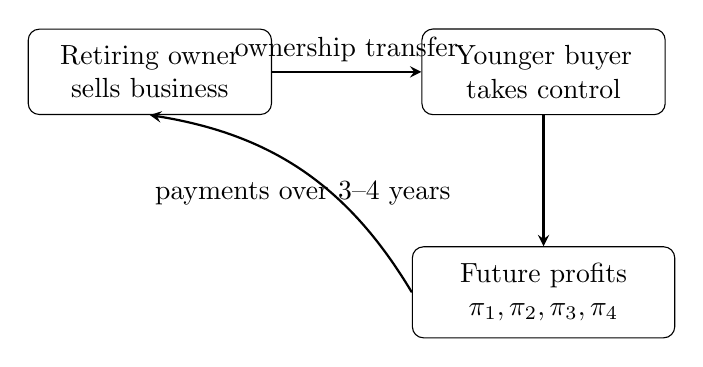
\begin{tikzpicture}[>=stealth, node distance=2.8cm]
\node[draw, rounded corners, align=center, inner sep=6pt, text width=0.22\textwidth] (seller) {Retiring owner\\sells business};
\node[draw, rounded corners, align=center, inner sep=6pt, text width=0.22\textwidth, right of=seller, xshift=2.2cm] (buyer) {Younger buyer\\takes control};
\node[draw, rounded corners, align=center, inner sep=6pt, text width=0.24\textwidth, below of=buyer] (profits) {Future profits\\\(\pi_1,\pi_2,\pi_3,\pi_4\)};
\draw[->, thick] (seller) -- node[above]{ownership transfer} (buyer);
\draw[->, thick] (buyer) -- (profits);
\draw[->, thick] (profits.west) to[bend right=25] node[below]{payments over \(3\)--\(4\) years} (seller.south);
\end{tikzpicture}
\caption{A transcript-based sketch of the vendor-finance mechanism.}
\end{figure}

The lecture does not stop at operational advice. It returns to the question of tax and makes a moral claim. Harpin says that he paid nearly \(\pounds 100\) million in tax when he sold HomeServe, that it was worth it because he made a great deal of money, and that billionaires should pay their taxes so long as the tax regime remains relatively low and affordable. The lecture is careful in its own way: it is neither celebrating confiscation nor preaching pure escape. It is arguing that large enterprise and civic contribution can coexist.

\section{Interlude, Timing, and Proximity}

After Harpin the lecture briefly turns outward and advertises further access. The host presents future conversations with founders and investors using the same kind of numerical bait that structured the opening montage: a healthcare company sold for \(\$460\) million, a beverage company reportedly taken from zero to \(\$500\) million in less than five years and then sold to Pepsi for \(\$2\) billion, and a private-equity billionaire who buys and scales companies. The interlude is not the conceptual center of the lecture, but it preserves the rhythm: after the strongest authority figure, the host pauses, recaps the scale, and then relaunches.

When the lecture returns to the street, it does so with a different mechanism in view. The Russian entrepreneur does not begin with copying a model. He begins with macro history. The Soviet Union collapsed when he was \(17\). Trade became possible. Oil prices rose. Mobile phones became popular. The money, in his telling, was made by catching a wave rather than by inventing a new physical law of business.

The key number in this segment is stated as revenue:
\begin{equation}
R_{2008} \approx \$5\times 10^9.
\end{equation}
This label matters. Revenue is not profit, and it is not personal net worth. The transcript is explicit about the category, and the notes should be equally explicit.

The lecture then adds two further elements. First, it returns to books. Asked what message he would leave to the younger generation, the entrepreneur says simply: read the books. When pressed further, he names \emph{Atlas Shrugged} and glosses it as a book about capitalism. Second, he offers a compressed masterclass on money: be in the right place, look at the expensive cars around you, understand that already-rich people cluster spatially, carry the right assortment, and motivate your team.

The host then performs one of his characteristic recap moves and extracts the principle in a sharper form: proximity is power. The faster one can follow the money, the faster one can reach it. Whatever we think of the slogan, it is an honest summary of the geometry that has governed the lecture from the move to Mayfair onward.

\section{Cost, Family, and Jurisdiction}

The final interview closes the chapter by combining three things the earlier sections kept partly separate: scale, arithmetic, and jurisdiction. The speaker begins with a family business in offshore energy and marine services, then explains that the original business was sold and a second iteration was later built. When the host pushes him numerically from ``a substantial nine-digit number'' up through \(\$900\) million to ``double that,'' the lecture lands on a very explicit arithmetic recognition:
\begin{equation}
1.8\times 10^9 = 1{,}800{,}000{,}000.
\end{equation}
That is why the host calls it a ten-digit number. The point here is not deep mathematics. It is that the lecture likes to turn scale into countable form whenever it can.

The same interview then supplies the cleanest local equation in the whole chapter. The father's business advice is not to focus on how much one sells for, but on underlying cost. We therefore write
\begin{equation}
m=p-c,
\end{equation}
where \(p\) is the selling price, \(c\) the unit cost, and \(m\) the unit margin.

\begin{proposition}
For a fixed menu of attainable sale prices \(p_1,\dots,p_k\), lowering unit cost from \(c\) to \(c'<c\) raises every corresponding margin by the same amount \(c-c'\).
\end{proposition}

\begin{proof}
If \(m_i=p_i-c\) and \(m_i'=p_i-c'\), then
\[
m_i'-m_i = (p_i-c')-(p_i-c)=c-c'>0.
\]
So every admissible sale price becomes more profitable by the same additive amount.
\end{proof}

The lecture immediately illustrates this with numbers rather than abstractions. If the product sells for \(\$10\) and costs \(\$8\), then
\begin{equation}
m(10,8)=10-8=2.
\end{equation}
Now lower the cost base to \(\$2\). Then
\begin{align}
m(5,2)&=5-2=3,\\
m(7,2)&=7-2=5,\\
m(10,2)&=10-2=8.
\end{align}
This is a small piece of algebra, but it does real work. The lesson is not simply that higher margins are nicer. It is that lower costs widen the range of market conditions under which one can still trade.

\paragraph{Worked derivation.}
\begin{enumerate}
\item Begin with the identity \(m=p-c\).
\item Fix the initial sale price at \(p=10\) and the initial cost at \(c=8\).
\item Compute the first margin: \(m=2\).
\item Lower the cost to \(c=2\).
\item Recompute the margin at several possible sale prices \(p=5,7,10\).
\item Observe that lower cost creates pricing freedom: one can accept lower market prices while keeping the business viable.
\end{enumerate}

The interview then returns to the human side of enterprise. Working with family is described as genuinely difficult. The father had to stop seeing the son only as a son; the son had to learn that harsh criticism in business was not identical with personal injury. The lecture is therefore careful here too. Family business is not romanticized. It is treated as a structure with its own friction.

Finally the lecture comes back to taxes, but now the answer is not moral first. It is structural first. The speaker says he is resident in the UAE and implies that this residence shaped the tax consequences of the exit. This is the lecture's last major variation on the title theme: perhaps the relevant question is not only whether a billionaire pays taxes, but where the billionaire is located when the taxable event occurs.

\subsection{Question \& Answer}

\paragraph{Question.} Does the lecture end with a single doctrine about whether billionaires pay taxes?

\paragraph{Answer.} No. It ends with a contrast that the chapter should keep alive. Harpin says that he paid nearly \(\pounds 100\) million in tax and treats that payment as part of the social compact of making a great deal of money. The final interviewee treats tax exposure as strongly shaped by jurisdiction and residence, and he describes the UAE as a place whose legal structure changes the outcome. The lecture does not resolve this contrast into a theorem. It leaves us with a productive tension between ethics and structure.

\section{Summary}

The lecture begins as spectacle and becomes, step by step, a set of commercial mechanisms. First we are given a tax heuristic and a city: London, rich and heavily taxed. Then we are shown that access to rich subjects is itself hard, which justifies the move to Mayfair. The jeweler teaches the linkage between hustle, trust, luxury-cycle timing, and expense. Harpin supplies the lecture's most formal object, an ordered nine-step sequence, and pairs it with a defense of paying taxes. The Russian entrepreneur adds macro timing, popularity, reading, and proximity. The final family-business interview closes the circle with clean margin arithmetic and a jurisdictional answer to the tax problem.

There is no blackboard here, but there is still structure. Revenue is not earnings, earnings are not valuation, valuation is not tax paid, and tax paid is not identical with either virtue or exploitation. Once we keep those distinctions steady, the lecture ceases to be a pile of expensive anecdotes and becomes something more useful: a guided tour through the arithmetic, geometry, and rhetoric of wealth under taxation.